% -- Encoding UTF-8 without BOM
% -- XeLaTeX => PDF (BIBER)

\documentclass{cv-style}     % Add 'print' as an option into the square bracket to remove colours from this template for printing.

\setdefaultlanguage{french}
\sethyphenation{french}{} % Add words between the {} to avoid them to be cut

%----------------------------------------------------------------------------------------
%	Page layout
%----------------------------------------------------------------------------------------
\cvheadheight{3.5cm}
\cvasidewidth{4.7}
\cvasidevpos{3.5}
\cvmainwidth{11.5cm}
\geometry{left=6.4cm, top=2.5cm, right=1cm, bottom=1cm}

%----------------------------------------------------------------------------------------
%	hyperlink setup
%----------------------------------------------------------------------------------------
\hypersetup{
    pdftitle=CV \textbar{} Laura Gomez,%
    pdfauthor=Laura Gomez
}

%----------------------------------------------------------------------------------------
%	Setup las updated text
%----------------------------------------------------------------------------------------
%\lastupdated{Mise à jour le \today}

%----------------------------------------------------------------------------------------
%	Add a few custom packages
%----------------------------------------------------------------------------------------
\usepackage{fontawesome}

\begin{document}

\header{Laura }{Gomez}{Chef de projet technique en mécatronique et biomécanique}         % Your name
%\lastupdated

%----------------------------------------------------------------------------------------
%	SIDEBAR SECTION  -- In the aside, each new line forces a line break
%----------------------------------------------------------------------------------------

\begin{aside}
    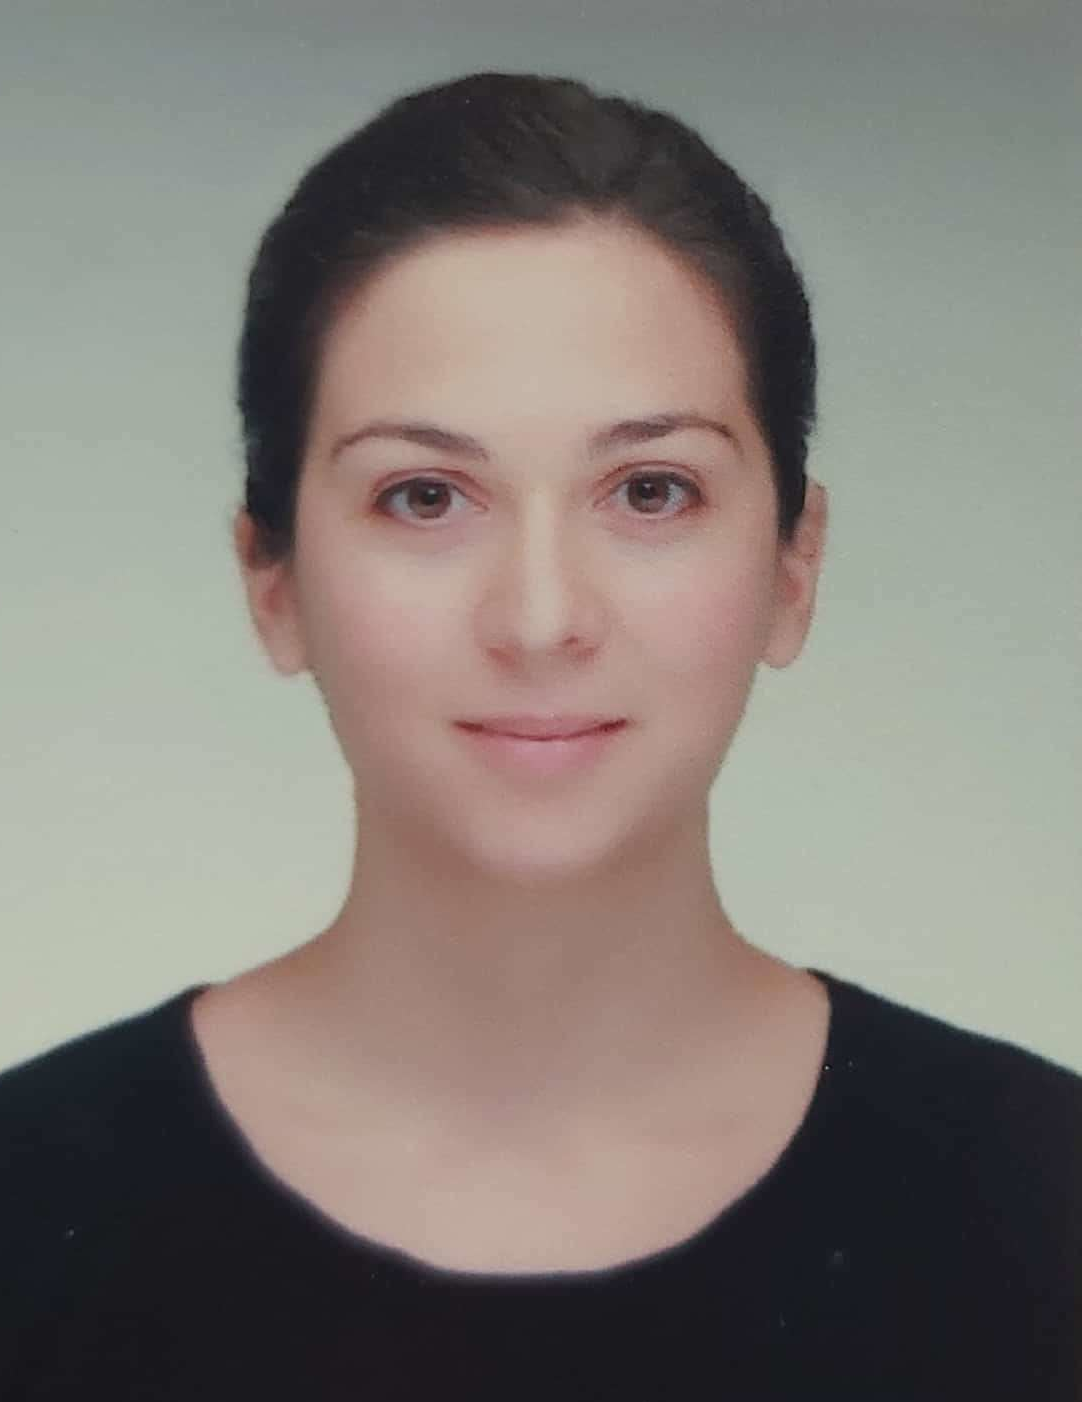
\includegraphics[width=.8\columnwidth]{img/LG}
    %\textbf{Disponibilité immédiate}
    91 rue du Colonel Fabien
    92160 Antony
    France
    ~
    Nationalité Française
    13 janvier 1989, France
    En concubinage
    Permis B
    %
    \section{Contact}
    laura-gomez@gmx.fr
    +33 7 70 49 23 44
    %
    \section{Gestion de projet}
    Microsoft Office
    ERP (Dolibarr, Sage)
    Gestion des exigences (IBM DOORS, Reqtify)
    ~
    Rédaction brevet
    Suivi Marquage règlementaire
    Suivi de la documentation
    %
    \section{Logiciel}
    C, Matlab
    Systèmes embarqués %(Arduino, Mbed)

    CAO %(Solidworks, Fusion360, OpenSim)

    Simulation multiphysique %(Flotherm)
    Conception Electronique %(Simulink, Labview, Zuken, Altium) 
    Outils d’étude du movement humain %(Nexus pour Vicon, MT Manager pour Xsens (centrales inertielles))
    %
    \section{Langues}
    Français (langue maternelle)
    Anglais (courant)
    Espagnol (courant)
    %
    \section{Soft Skills}
    Autonome et proactive
    Pensée analytique
    Bon esprit d'équipe
    %
    \section{Hobbies}
    Violoncelle et orchestre
    Vélo et course à pied
    %
\end{aside}

\section{Rés}{umé}

Mécatronicienne de formation, j’ai eu l’occasion de piloter le développement matériel et logiciel de produits, 
dès leur phase de développement et jusqu'à leur industrialisation. Il m'a également été donné de pouvoir piloter la mise en conformité de produits 
déjà existants afin qu'ils répondent aux besoins spécifiques du client.
Dans ce contexte, j'ai assuré une bonne communication entre toutes les parties prenantes internes et externes concernées, 
afin de respecter les délais et la qualité du produit final.
D'une grande capacité d'adaptation, j’aime apprendre au quotidien et partager mes connaissances avec mes collègues.


\section{Experience}{ Professionnelle}

\begin{entrylist}
%------------------------------------------------
\entry
  {2021}
  {NeoFarm}
  {Robotique maraichère}
  {\jobtitle{Ingénieure mécatronique, Ingénieure industrialisation}\\
   Développements et tests d'outils maraichers adaptés au robot

   Suivi fournisseurs

   Suivi marquage réglementaire

   Mise en place ERP et règles de conception
   }
 
%------------------------------------------------
\entry
  {2020}
  {Safran}
  {Défense}
  {\jobtitle{Ingénieure système}\\
  Etude biomécanique

  Recueil et synthèse du besoin en provenance des diverses parties prenantes

  Recherche des solutions existantes sur le marché

  Suivi fournisseurs Français et étrangers

  Déclinaison d’exigences sous IBM DOORS 
  }
%------------------------------------------------
\entry
  {2018--2019}
  {Safran - Zodiac (prestation pour Alten)}
  {Aéronautique}
  {\jobtitle{Chef de projet technique de systèmes mécatronique}\\
  Recueil du besoin d'un client Italien

  Traduction du besoin en actions R\&D

  Gestion des échanges technique et documentaire entre le client et les différents BE

  Conception de harnais sous Zuken, travail avec l'équipe Production

  Essais du système chez le client
 
  }
%------------------------------------------------
\entry
 {2017--2018}
 {Air Liquide Medical System (prestation pour Ametra)}
 {Médical - ventilation}
 {\jobtitle{Référente mécanique - nouveau produit et plasturgie}\\
 En charge de l'évolution du système actuel pour réduire les fissures

 Suivi des échantillons initiaux de la coque plastique d'un nouvel appareil

 Suivi des plasturgistes

 8D
 }
%------------------------------------------------
\entry
 {2016}
 {CEA (intérim pour Manpower)}
 {Cobotique Agro-alimentaire}
 {\jobtitle{Chef de projet technique de systèmes cobotique}\\
 Etude du besoin au poste de travail (biomécanique)

 Recherche de solutions, conception, fabrication de démonstrateurs

 Essais des prototypes par les opérateurs

 Rédaction de brevets
 }
%------------------------------------------------

\end{entrylist}

%----------------------------------------------------------------------------------------
%	EDUCATION SECTION
%----------------------------------------------------------------------------------------

\section{Form}{ation}

\begin{entrylist}
%--------------------------------------G----------
\entry
{2013--2015}
{Master recherche d'ingénierie biomédical {\normalfont spécialité biomécanique}}
{BME et Arts et Métiers, France}
{Master international}
%------------------------------------------------
\entry
{2008--2013}
{Ecole d'ingénieur en mécatronique {\normalfont spécialité robotique et simulation}}
{ISTY - UVSQ}
{6 mois en Corée à l'Université Ajou}
\end{entrylist}

\end{document}
